\documentclass{beamer}
\usetheme{tokitex}

\usepackage{graphics}
\usepackage{multirow}
\usepackage{tabto}

\usepackage[english,bahasa]{babel}
\newtranslation[to=bahasa]{Section}{Bagian}
\newtranslation[to=bahasa]{Subsection}{Subbagian}

\usepackage{listings, lstautogobble}
\usepackage{color}

\definecolor{dkgreen}{rgb}{0,0.6,0}
\definecolor{gray}{rgb}{0.5,0.5,0.5}
\definecolor{mauve}{rgb}{0.58,0,0.82}

\lstset{frame=tb,
  language=pascal,
  aboveskip=1mm,
  belowskip=1mm,
  showstringspaces=false,
  columns=fullflexible,
  keepspaces=true,
  basicstyle={\small\ttfamily},
  numbers=none,
  numberstyle=\tiny\color{gray},
  keywordstyle=\color{blue},
  commentstyle=\color{dkgreen},
  stringstyle=\color{mauve},
  breaklines=true,
  breakatwhitespace=true,
  autogobble=true
}

\title{Struktur Data Dasar}
\author{Tim Olimpiade Komputer Indonesia}
\date{}

\begin{document}

\begin{frame}
\titlepage
\end{frame}

\begin{frame}
\frametitle{Pendahuluan}
Melalui dokumen ini, kalian akan:
\begin{itemize}
	\item Mengenal beberapa macam struktur data dasar
	\item Mengetahui pentingnya penggunaan struktur data
	\item Mengetahui operasi-operasi yang dapat dilakukan pada struktur data dasar
\end{itemize}
\end{frame}

\begin{frame}
\frametitle{Kilas Balik: Array}
Apakah Anda masih ingat mengenai struktur data array?
Array merupakan salah satu contoh struktur data yang dasar yang mendukung operasi berikut :
\begin{itemize}
	\item Membaca elemen didalam array secara random. Pada array, kita dapat membaca elemen pada indeks yang kita inginkan.
	\item Mengupdate elemen didalam array secara random. Pada array, kita dapat mengubah nilai elemen didalam array
\end{itemize} 
\end{frame}

\section{Linked List}
\frame{\sectionpage}

\begin{frame}
\frametitle{Mengenal Linked List}
\begin{figure}
	\centering
	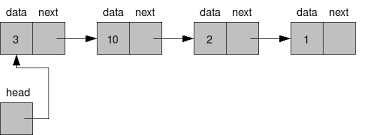
\includegraphics[width=6 cm]{asset/linkedlist.png}
\end{figure}
\begin{itemize}
	\item Linked list terdiri dari kumpulan \alert{node} yang saling terhubung
	\item Tiap node terdiri dari elemen yang akan disimpan dan \alert{pointer} ke node lainnya
	\item Pointer tersebut yang menghubungkan antar node dalam linked list
\end{itemize}
\end{frame}

\begin{frame}
\frametitle{Mengenal Linked List (lanj.)}
Berdasarkan hubungannya dengan node lain, linked list terbagi menjadi 2 macam, yaitu:
\begin{itemize}
	\item Single Linked List, yaitu linked list dimana tiap nodenya hanya memiliki pointer ke node selanjutnya saja. Tiap node hanya memiliki pointer \alert{next} untuk menunjuk node selanjutnya.
	\item Double Linked List, yaitu linked list dimana tiap nodenya memiliki pointer terhadap node selanjutnya dan node sebelumnya. Tiap pointer memiliki pointer next dan \alert{prev} untuk menunjuk node sebelumnya.
\end{itemize}
\end{frame}

\begin{frame}
\frametitle{Mengenal Linked List (lanj.)}
Selain itu, berdasarkan bentuknya, linked list juga dapat terbagi menjadi 2 macam, yaitu:
\begin{itemize}
	\item Linear Linked List, yaitu linked list dimana \alert{tail} atau node paling terakhir nextnya dihubungkan ke \alert{NULL}. Demikian pula dalam double linked list, maka \alert{head} atau node pertama prevnya dihubungkan ke NULL.
	\item Circular Linked List, yaitu linked list dimana tail bagian nextnya akan dihubungkan ke head. Selain itu, bagian prev pada head juga akan dihubungkan ke tail. 
\end{itemize}
\end{frame}

\begin{frame}
\frametitle{Keuntungan Linked List}
Mengapa kita harus menggunakan linked list? Hal ini dikarenakan linked list memiliki keuntungan dalam menangani penghapusan suatu elemen. Sebagai contoh, misal kita akan menghapus salah satu elemen pada linked list. Maka yang perlu dilakukan hanya menghapus node tersebut. Jika dibandingkan dengan array, maka penghapusan suatu elemen harus menggeser seluruh elemen setelah atau sebelum elemen yang dihapus.
\end{frame}

\begin{frame}
\frametitle{Kerugian Linked List}
Namun, penggunaan linked list juga memiliki kerugian. Sebagai contoh, untuk proses membaca elemen tidak semudah dalam pembacaan elemen pada array. Untuk membaca elemen pada indeks tertentu, maka harus dilakukan iterasi mulai dari node head hingga ke node yang diinginkan. Begitu pula dengan proses pengupdatean harus dilakukan iterasi dari awal terlebih dahulu.
\end{frame}

\section{Stack}
\frame{\sectionpage}

\begin{frame}
\frametitle{Soal Pemanasan}

Misal kita mendapat soal sebagai berikut
\begin{itemize}
	\item Anda diberikan sebuah string misal "acaabcbcd"
	\item Cari string "abc" dalam string tersebut. Jika ditemukan maka hapus string "abc" tersebut, lalu ulangi pencarian.
	\item Pencarian berakhir ketika tidak terdapat string "abc" lagi. Outputkan total penghapusan yang berhasil dilakukan
	\item Contoh, pada string "acaabcbcd" terdapat sebuah string abc, dan hapus string tersebut menjadi "acabcd". Lalu, ditemukan lagi string abc dan hapus menjadi "acd". Karena tidak ditemukan lagi string "abc", maka output 2.
\end{itemize}
\end{frame}

\begin{frame}
\frametitle{Mengenal Stack}

Stack dapat dimisalkan seperti tumpukan piring. Jika terdapat piring baru yang ingin dimasukkan, maka piring tersebut masuk dari paling atas. Jika sebuah piring akan diambil dari tumpukan, maka yang diambil juga piring yang paling atas.

\begin{figure}
	\centering
	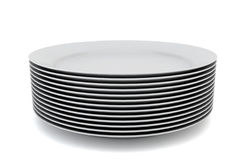
\includegraphics[width=4 cm]{asset/plates-stack.jpg}
\end{figure}

\end{frame}

\begin{frame}
\frametitle{Mengenal Stack (lanj.)}

Seperti pada analogi tumpukan piring, struktur data stack memiliki sifat yang sama:
\begin{itemize}
	\item Push, yaitu memasukan elemen baru ke bagian akhir dari stack
	\item Pop, yaitu membuang elemen paling akhir dari stack
\end{itemize}

\begin{figure}
	\centering
	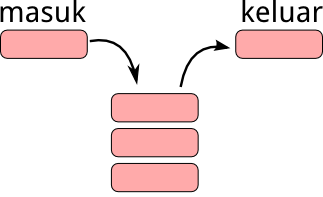
\includegraphics[width=4 cm]{asset/stack.png}
\end{figure}
\end{frame}

\begin{frame}
\frametitle{Pembahasan Soal}

Setelah mengenali struktur data stack, maka kita sudah dapat menjawab soal sebelumnya dengan efisien.
\begin{itemize}
	\item Lakukan iterasi tiap karakter pada string tersebut
	\item Untuk karakter selain huruf 'c', maka masukkan ke stack yang dimiliki
	\item jika karakter sekarang adalah 'c', maka ada kemungkinan bahwa string terakhir adalah "abc". Oleh karena itu, cek 2 elemen teratas dari stack, apakah 'b' dan 'a'.
	\item Jika tidak, maka masukkan 'c' kedalam stack.
	\item Jika iya, maka terdapat 1 penghapusan, lalu pop huruf 'b' dan 'a' dari stack.
\end{itemize}
Kompleksitas total adalah O(n) yang cukup efisien karena pada tiap karakter, kita hanya memasukkan kedalam stack atau mengecek 2 elemen teratas dari stack.
\end{frame}

\section{Queue}
\frame{\sectionpage}

\begin{frame}
\frametitle{Mengenal Queue}

Apakah anda pernah melihat antrian pembelian? Tentu saja pernah bukan?
\newline
\newline
Struktur Data Queue mirip dengan analogi antrian tersebut. Saat seorang ingin masuk ke antrian, maka orang tersebut harus mengantri dari belakang. Sementara itu, orang yang dilayani terlebih dahulu adalah orang yang paling depan.

\begin{figure}
	\centering
	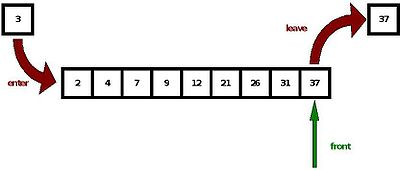
\includegraphics[width=6 cm]{asset/queue.jpg}
\end{figure}
\end{frame}

\begin{frame}
\frametitle{Mengenal Queue (lanj.)}

Setelah mengenal struktur data queue, berikut adalah beberapa operasi yang dapat dilakukan oleh queue :
\begin{itemize}
	\item Push, yaitu memasukkan elemen baru kedalam indeks paling akhir dari queue
	\item Pop, yaitu mengeluarkan elemen paling depan dari queue
	\item Front, yaitu melihat elemen yang paling depan dari queue tersebut
\end{itemize}
\end{frame}

\section{Binary Search Tree}
\frame{\sectionpage}

\begin{frame}
\frametitle{Soal Pemanasan}
Misalkan Anda diberi problem dimana terdapat 2 macam query, yaitu insert suatu angka dan cari suatu angka. Perintah insert adalah memasukan angka tersebut ke struktur data. Perintah cari berarti mencari angka yang diinput dalam struktur data yang ada. Jika angka tersebut ada, print 1, jika tidak ada print 0.
\newline\newline
Cara yang paling mudah adalah untuk tiap operasi insert, maka masukkan angka tersebut ke array indeks paling akhir. Lalu, untuk operasi cari, maka lakukan linear search pada array. Namun, operasi pencarian ini kurang efisien karena butuh O(n) untuk mencari angka tersebut.
\end{frame}

\begin{frame}
\frametitle{Mengenal Binary Search Tree}
Untuk memperkecil kompleksitas problem tersebut, maka kita perlu belajar mengenai Binary Search Tree. Binary Search Tree merupakan struktur data yang cukup berbeda dengan struktur data yang sebelumnya. Berikut adalah ilustrasi sekilas mengenai binary search tree

\begin{figure}
	\centering
	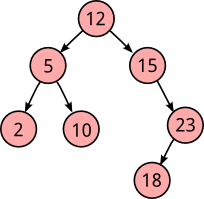
\includegraphics[width=4 cm]{asset/bst.png}
\end{figure}
\end{frame}

\begin{frame}
\frametitle{Mengenal BST (lanj.)}
Berdasarkan ilustrasi diatas, maka dapat disimpulkan beberapa hal berikut:
\begin{itemize}
	\item Tiap node pada BST memiliki sebuah nilai dan 2 pointer ke anaknya (anak kiri dan anak kanan).
	\item Node yang berada di sebelah kiri suatu node pasti memiliki nilai yang lebih kecil daripada node sekarang.
	\item Node yang berada di sebelah kanan suatu node pasti memiliki nilai yang lebih besar daripada node sekarang.
	\item Node yang paling atas merupakan node \alert{root} yang merupakan satu-satunya node yang dapat diakses secara langsung
\end{itemize}
\end{frame}

\begin{frame}
\frametitle{Operasi Insert pada BST}

Dengan adanya sifat-sifat BST di atas, maka proses insert dapat dimulai dari node root. Lakukan hal berikut hingga menemukan node NULL.
\begin{itemize}
	\item Jika nilai pada node sekarang lebih besar daripada nilai yang akan diinsert, maka pergi ke anak kiri dari node sekarang.
	\item Jika nilai pada node sekarang lebih kecil dari nilai yang akan diinsert, maka pergi ke anak kanan dari node sekarang.\newline
\end{itemize}

Jika node sekarang NULL, maka buat node baru dengan anak kiri dan anak kanan adalah NULL. Jangan lupa untuk memasukkan nilai yang diinsert ke node tersebut.
\end{frame}

\begin{frame}[fragile]
\frametitle{Pseudocode Insert pada BST}

\begin{lstlisting}

node* insert (node* currNode, int value)

    if currNode = NULL:
        currNode = new Node
        currNode.val = value
        currNode.left_child = NULL
        currNode.right_child = NULL
	
    else if currNode.val > value:
        currNode.left_child =
        insert(currNode.left_child, value)
	
    else:
        currNode.right_child = 
        insert(currNode.right_child, value)
		
    return currNode
		
\end{lstlisting}
\end{frame}

\begin{frame}
\frametitle{Operasi Find pada BST}

Dengan adanya sifat-sifat BST di atas, maka proses find dapat dimulai dari node root. Lakukan hal berikut hingga menemukan angka yang dicari atau menemukan node NULL.
\begin{itemize}
	\item Jika nilai pada node sekarang lebih besar daripada nilai yang akan diinsert, maka pergi ke anak kiri dari node sekarang.
	\item Jika nilai pada node sekarang lebih kecil dari nilai yang akan diinsert, maka pergi ke anak kanan dari node sekarang.\newline
\end{itemize}
Jika value dari node sekarang sesuai dengan yang dicari, berarti angka yang dicari ditemukan dalam BST.
\newline\newline
Jika node sekarang NULL, maka angka yang dicari tidak ditemukan dalam BST.
\end{frame}

\begin{frame}[fragile]
\frametitle{Pseudocode Insert pada BST}

\begin{lstlisting}

int insert (node* currNode, int value)

    if currNode = NULL:
        return 0
    
    else if currNode.val = value:
        return 1
        
    else if currNode.val > value:
        return insert(currNode.left_child, value)
        
    else:
        return insert(currNode.right_child,value)
		
\end{lstlisting}
\end{frame}

\begin{frame}
\frametitle{Pembahasan Soal}

Setelah mengenai BST, maka untuk menyelesaikan masalah sebelumnya kita dapat menggunakan BST. Untuk proses insert, maka gunakan proses insert yang terdapat pada BST. Untuk proses find, juga gunakan proses find yang terdapat pada BST.
\newline\newline
Dengan demikian, kompleksitas dari insert dan find keduanya adalah sesuai dengan tinggi dari BST. Solusi ini lebih efisien daripada menggunakan array dan harus mencari seluruh isi array
\end{frame}

\end{document}


